\documentclass[a4paper,12pt]{article}
\usepackage[utf8]{inputenc}
\usepackage[T1]{fontenc}
\usepackage[hungarian]{babel}
\usepackage{graphicx}
\usepackage{geometry}
\geometry{a4paper,
		     tmargin = 35mm, 
		     lmargin = 25mm,
		     rmargin = 30mm,
		     bmargin = 30mm}
\usepackage{mathtools}
\usepackage{amsmath}
\usepackage{color}
\usepackage{setspace}
\usepackage{amsmath,amssymb}
\usepackage{float}


\usepackage{indentfirst}
\usepackage{subfig}

\renewcommand\thesection{\Roman{section}}

\begin{document}

\linespread{1.2}

\begin{titlepage}

	\centering
	
\includegraphics[width=0.66\textwidth]{../elte.jpg}\par\vspace{1cm}
	{\scshape\LARGE ELTE TTK \par}
	\vspace{3cm}
	{\scshape\Large Pásztázó elektronmikroszkópia\par}
	\vspace{1cm}
	{\large\itshape Olar Alex\par}
	\vspace{3cm}
	{\large 2018 \par}

\end{titlepage}

\begin{abstract}
	\par A mérés célja a SEM mikroszkóppal való ismerkedés és a tapasztalat szerzés volt. Idén láthattuk, hogy
	a modern technika eliminálta a laborok eddigi legfontosabb részét, avagy az 50 éves műszer kalibrálását és
	kezelését. Láthattuk, hogy egy modern géppel, a modern szoftverek szinte mindent megcsinálnak helyettünk.
\end{abstract}

\vfill

\tableofcontents

\newpage

\section{Elméleti összefoglaló}

\par A pásztázó elektronmikroszkópia elmélete már korábbi tanulmányaink során előfordult és a leírásban
is szerepel. A képkészítéshez a műszer a szekunder elektronokat és a visszaszórodott elektronokat használta
és a képeket a megfelelő elektronika készítette el a műszerben lévő detektor segítségével.

\section{A mérés lépései}

\par A mérés során a modern műszer lehetőve tette, hogy mindhárman válasszunk egy mintát és azt megvizsgáljuk.
Megvizsgáltuk Dávid ezüst láncát és két micro chipet amik demonstrációs célra voltak fenntartva. Adott mintáról
készítettünk röntgen spektroszkópiai felvételeket is, melynek segítségével meg tudtuk határozni a kellő program
segítségével az anyagösszetételt és az összetétel arányt is a felszín közelében. Ezeket a képeket közlöm majd a
megfelelő táblázatokkal.

\par Előszöris persze egy három anyagból álló (szilícium-titán-réz/nikkel ötvözet) mintát vizsgáltunk a fentebbi
módszerekkel, hogy megismerjük a műszert és annak használatát.

\vfill

\newpage

\section{Mérési eredmények}

\subsection{Első minta}

\begin{figure}[H]
	\centering
	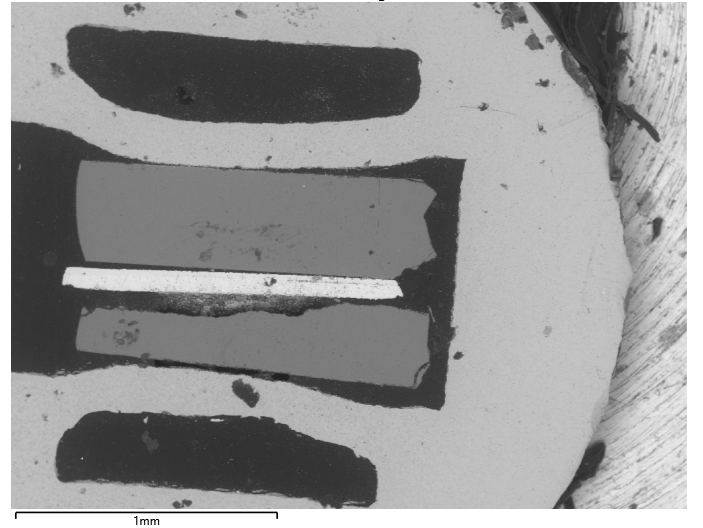
\includegraphics[width=0.35\textwidth, height=0.25\textwidth]{Jcsop/elso.png}
	\caption{Tanuló minta}
\end{figure}

\par A program által meghatározott anyagösszetétel is jól látható az alábbi ábrán. De a teljesség kedvéért
le is írom: Ni, Cu, Ti, Si, C.

\begin{figure}[H]
	\centering
	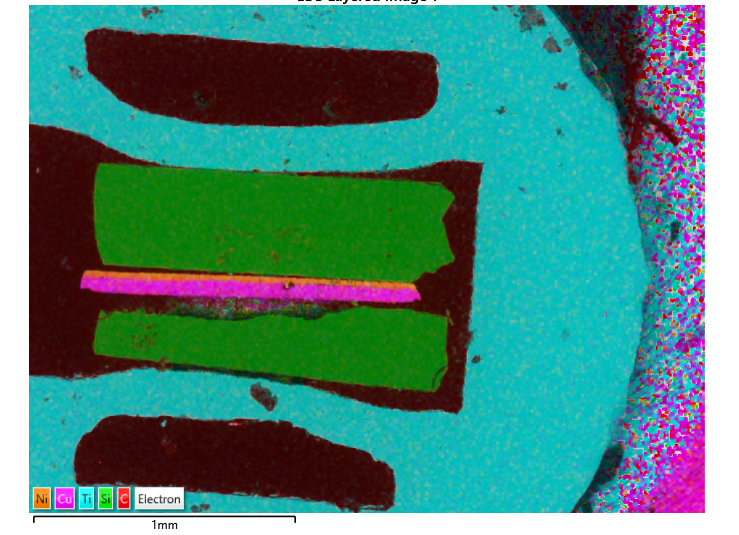
\includegraphics[width=0.65\textwidth, height=0.45\textwidth]{Jcsop/elsoanyag.png}
	\caption{Tanuló minta anyagösszetétele}
\end{figure}

\par Ugyan ezek az anyagok szépen szeparálódnak az egyenkénti röntgen felvételeken. A fentebbi kép ezek
szintetikus összerakásával készült:

\begin{figure}[H]
	\centering
	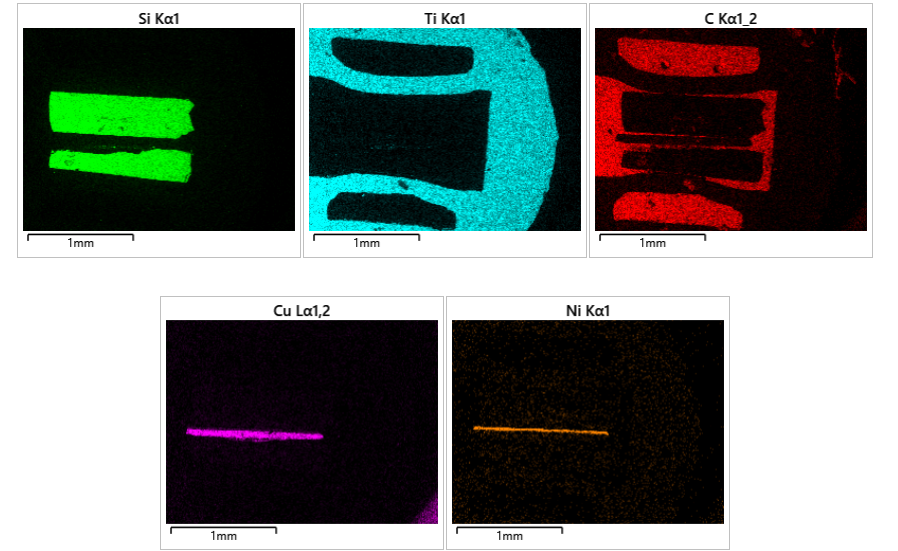
\includegraphics[width=0.65\textwidth, height=0.45\textwidth]{Jcsop/elsortg.png}
	\caption{Tanuló mintáról készült röntgen analízis}
\end{figure}

\subsubsection{Összetétel meghatározása}

\par Az alábbi mintáról a Cu L$\alpha$1,2 képet vizsgáltuk. A feladat
az volt, hogy a kapott képen márjük meg a különböző anyagok arányát (Cu-Ni-Si)
majd a készített hisztogrammon ezt ismételjük meg.

\begin{figure}[H]
	\centering
	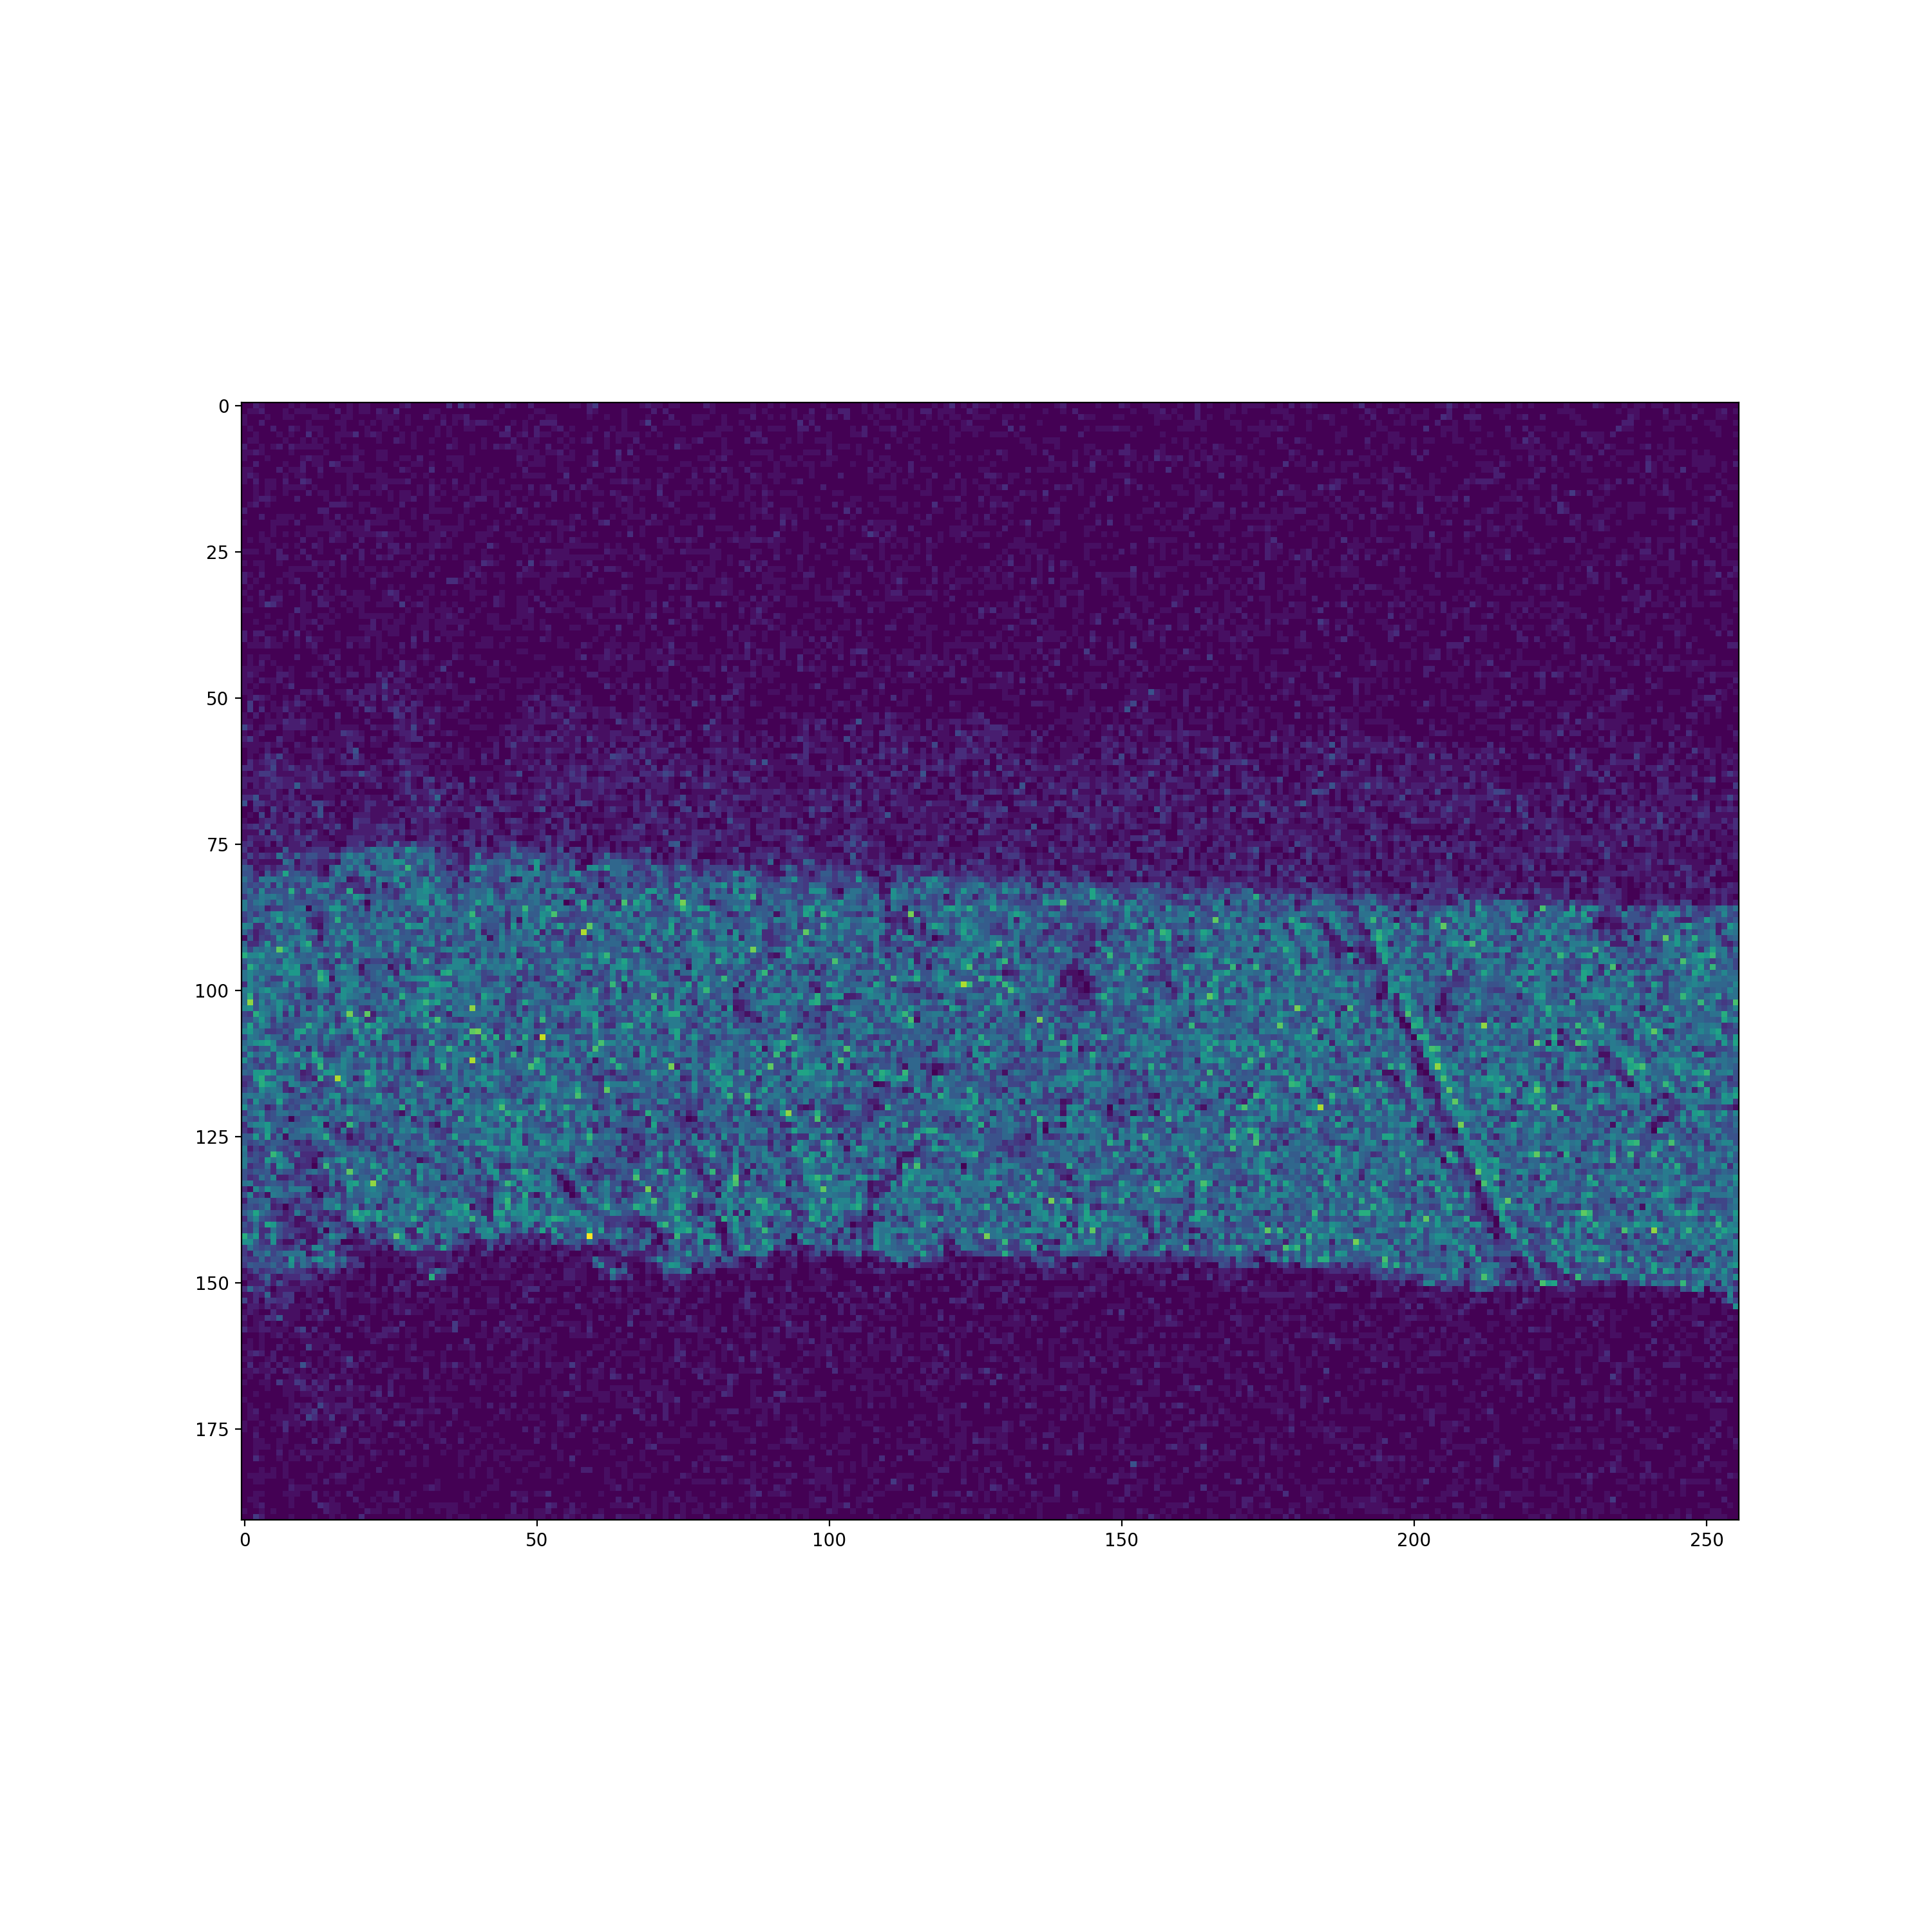
\includegraphics[width=0.52\textwidth]{histoimg.png}
	\caption{A vizsgált kép, a csv fájlból generálva.}
\end{figure}

\par A python matplotlib csomagjával az előbbi képből egy oszlop diagrammot
készítettem. Ennek a beosztását [0,20] közötti intervallumban vettem, hiszen a
kapott kép nem tartalmazott ennél nagyobb értékeket adott pixelben.

\begin{figure}[H]
	\centering
	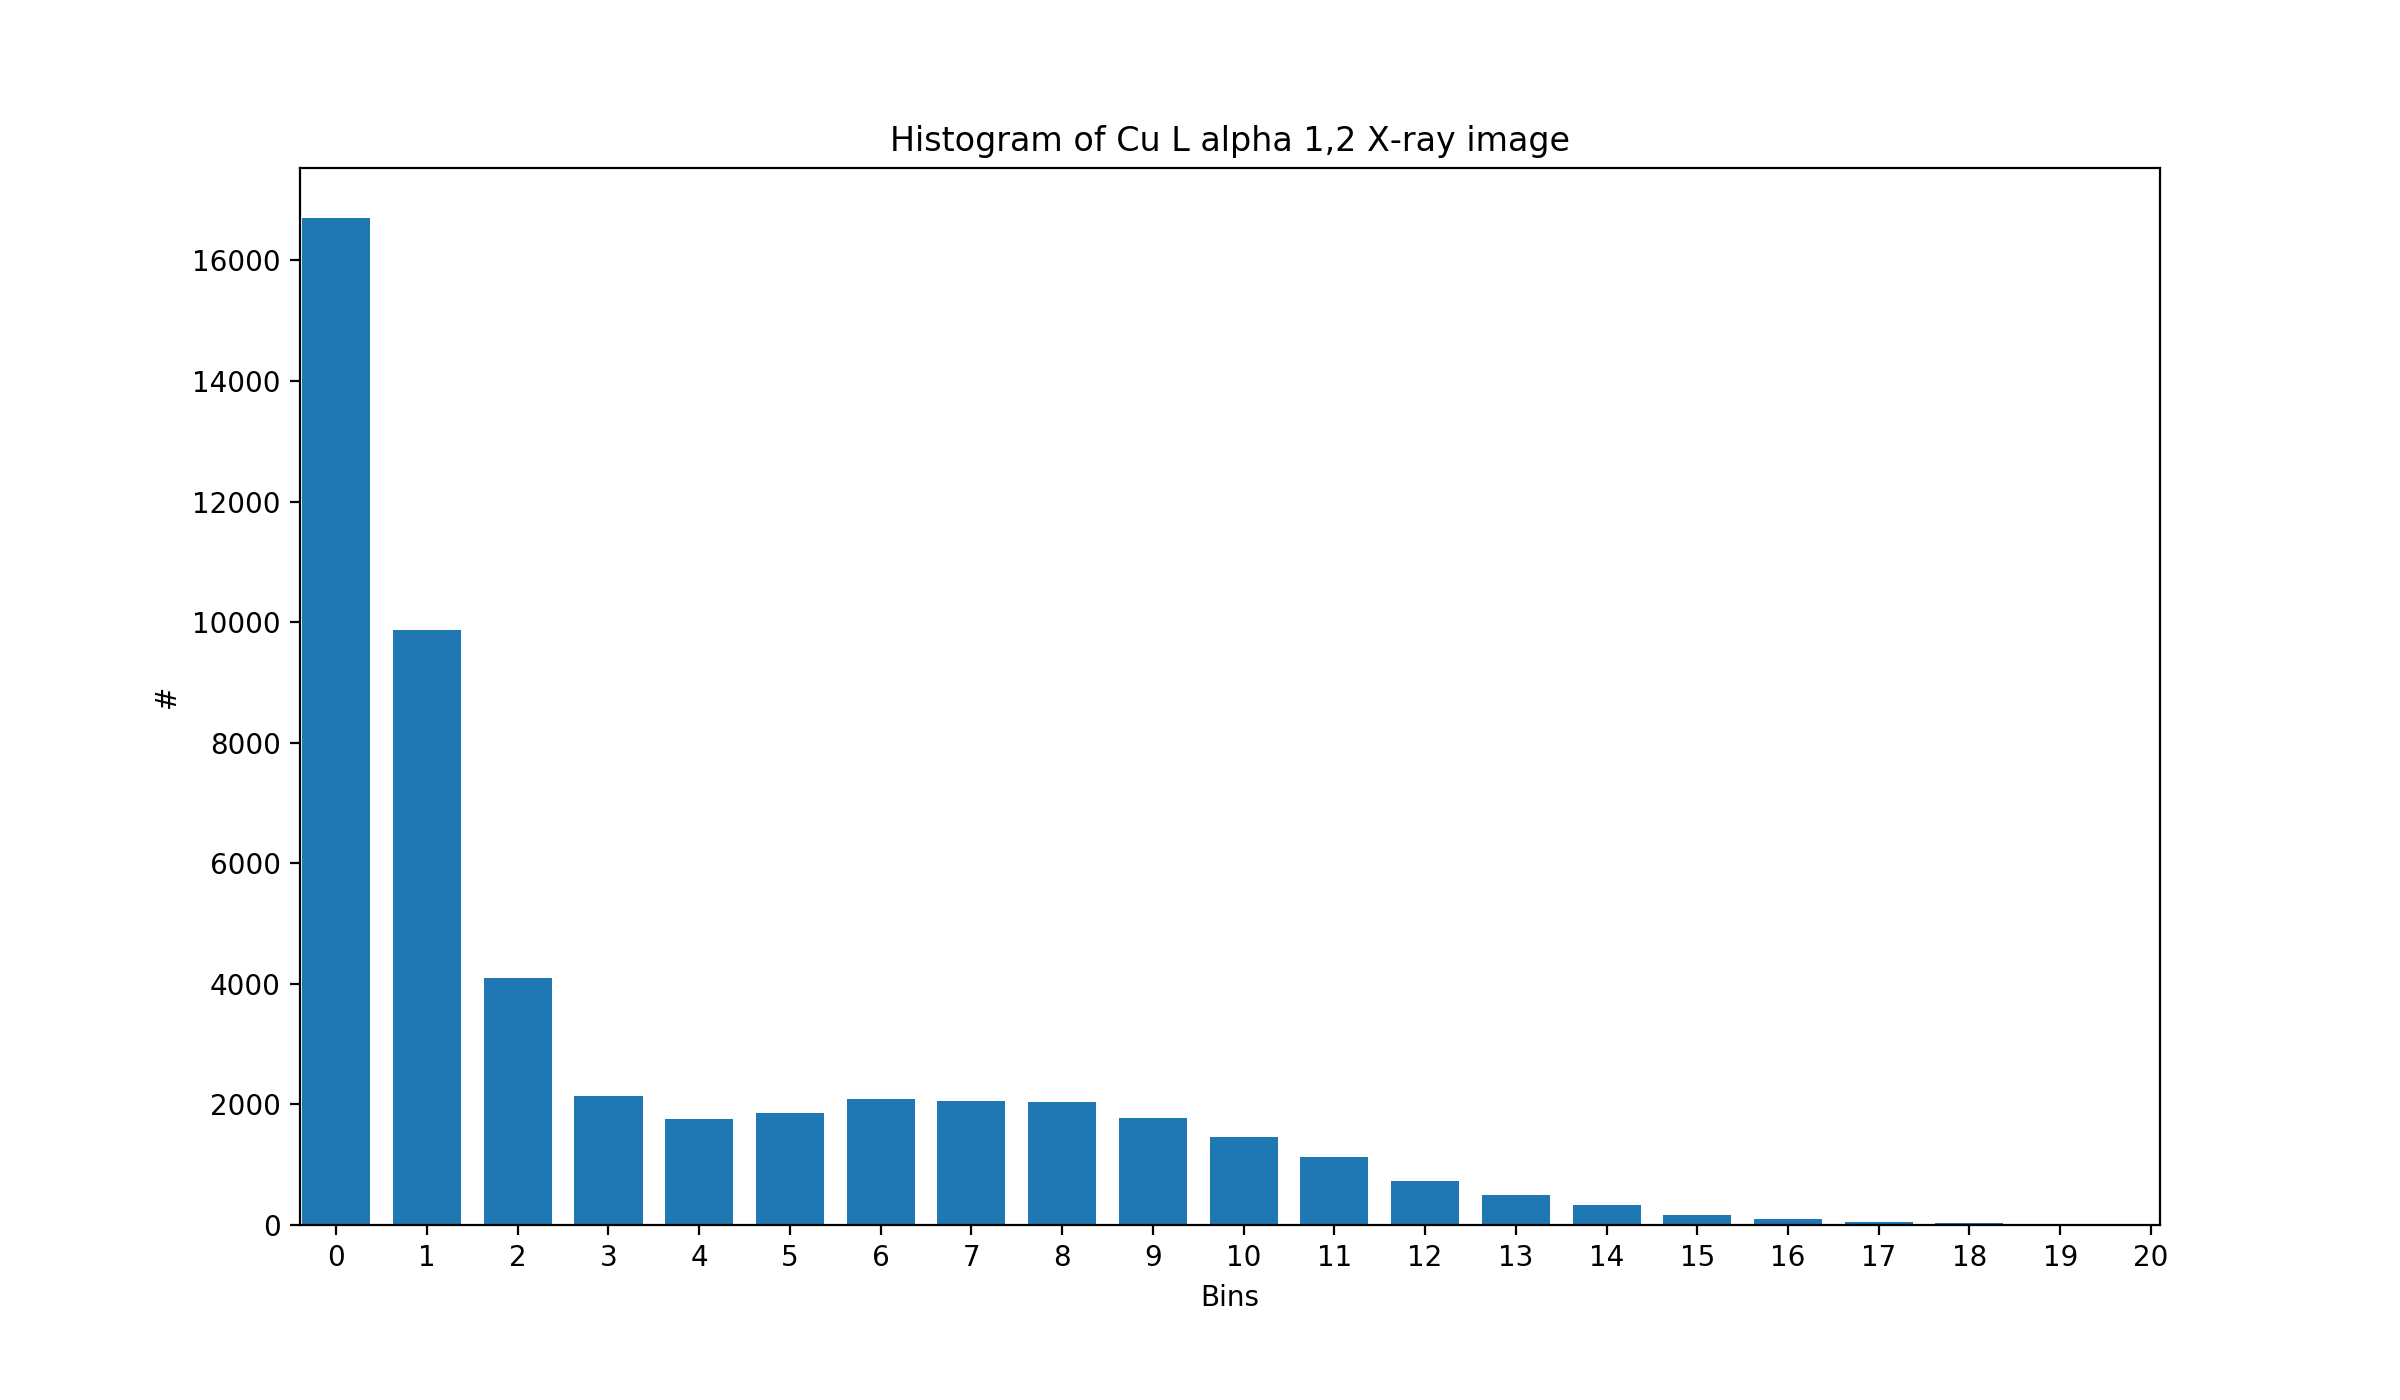
\includegraphics[width=0.82\textwidth]{histo.png}
	\caption{A kép hisztogrammon.}
\end{figure}

\par Jól látható, hogy a 192x256-os kép nagy része 0-ás értékű, ezeket veszem a legsötétebb
pontoknak. Nem jól elkülöníthatő a szemmel jól látható nikkel réteg a kép
közepe táján, ezt a kisebb csúcs előtti résznek veszem. Az eredmények a következők:



\section{Összefoglalás}

\par 

\end{document}